%%% Template originaly created by Karol Kozioł (mail@karol-koziol.net) and modified for ShareLaTeX use

\documentclass[a4paper,11pt]{article}

\usepackage[T1]{fontenc}
\usepackage[utf8]{inputenc}
\usepackage{graphicx}
\usepackage{xcolor}

\renewcommand\familydefault{\sfdefault}
\usepackage{tgheros}
% \usepackage[defaultmono]{droidmono}

\usepackage{amsmath,amssymb,amsthm,textcomp}
\usepackage{enumerate}
\usepackage{multicol}
\usepackage{tikz}

\usepackage{geometry}
\geometry{left=25mm,right=25mm,%
bindingoffset=0mm, top=20mm,bottom=20mm}


\linespread{1.3}

\newcommand{\linia}{\rule{\linewidth}{0.5pt}}

% custom theorems if needed
\newtheoremstyle{mytheor}
    {1ex}{1ex}{\normalfont}{0pt}{\scshape}{.}{1ex}
    {{\thmname{#1 }}{\thmnumber{#2}}{\thmnote{ (#3)}}}

\theoremstyle{mytheor}
\newtheorem{defi}{Definition}

% my own titles
\makeatletter
\renewcommand{\maketitle}{
\begin{center}
\vspace{2ex}
{\huge \textsc{\@title}}
\vspace{1ex}
\\
\linia\\
\@author \hfill \@date
\vspace{4ex}
\end{center}
}
\makeatother
%%%

% custom footers and headers
\usepackage{fancyhdr}
\pagestyle{fancy}
\lhead{}
\chead{}
\rhead{}
\lfoot{Report.Project.cuda }
\cfoot{}
\rfoot{Page \thepage}
\renewcommand{\headrulewidth}{0pt}
\renewcommand{\footrulewidth}{0pt}
%

% code listing settings
\usepackage{listings}
\lstset{
    language=Python,
    basicstyle=\ttfamily\small,
    aboveskip={1.0\baselineskip},
    belowskip={1.0\baselineskip},
    columns=fixed,
    extendedchars=true,
    breaklines=true,
    tabsize=4,
    prebreak=\raisebox{0ex}[0ex][0ex]{\ensuremath{\hookleftarrow}},
    frame=lines,
    showtabs=false,
    showspaces=false,
    showstringspaces=false,
    keywordstyle=\color[rgb]{0.627,0.126,0.941},
    commentstyle=\color[rgb]{0.133,0.545,0.133},
    stringstyle=\color[rgb]{01,0,0},
    numbers=left,
    numberstyle=\small,
    stepnumber=1,
    numbersep=10pt,
    captionpos=t,
    escapeinside={\%*}{*)}
}

%%%----------%%%----------%%%----------%%%----------%%%

\begin{document}

\title{Report.Project }

\author{Nguyen Ngoc Son 009, M2-ICT USTH}

\date{08/01/2023}

\maketitle

\section*{Summary}


In this lab work, CPU and 2D GPU parallelism are implemented with Kuwahara filter. The framework used is numba in python under Google Colab GPU session (Tesla GPU).

\begin{figure}[h]
    \centering
    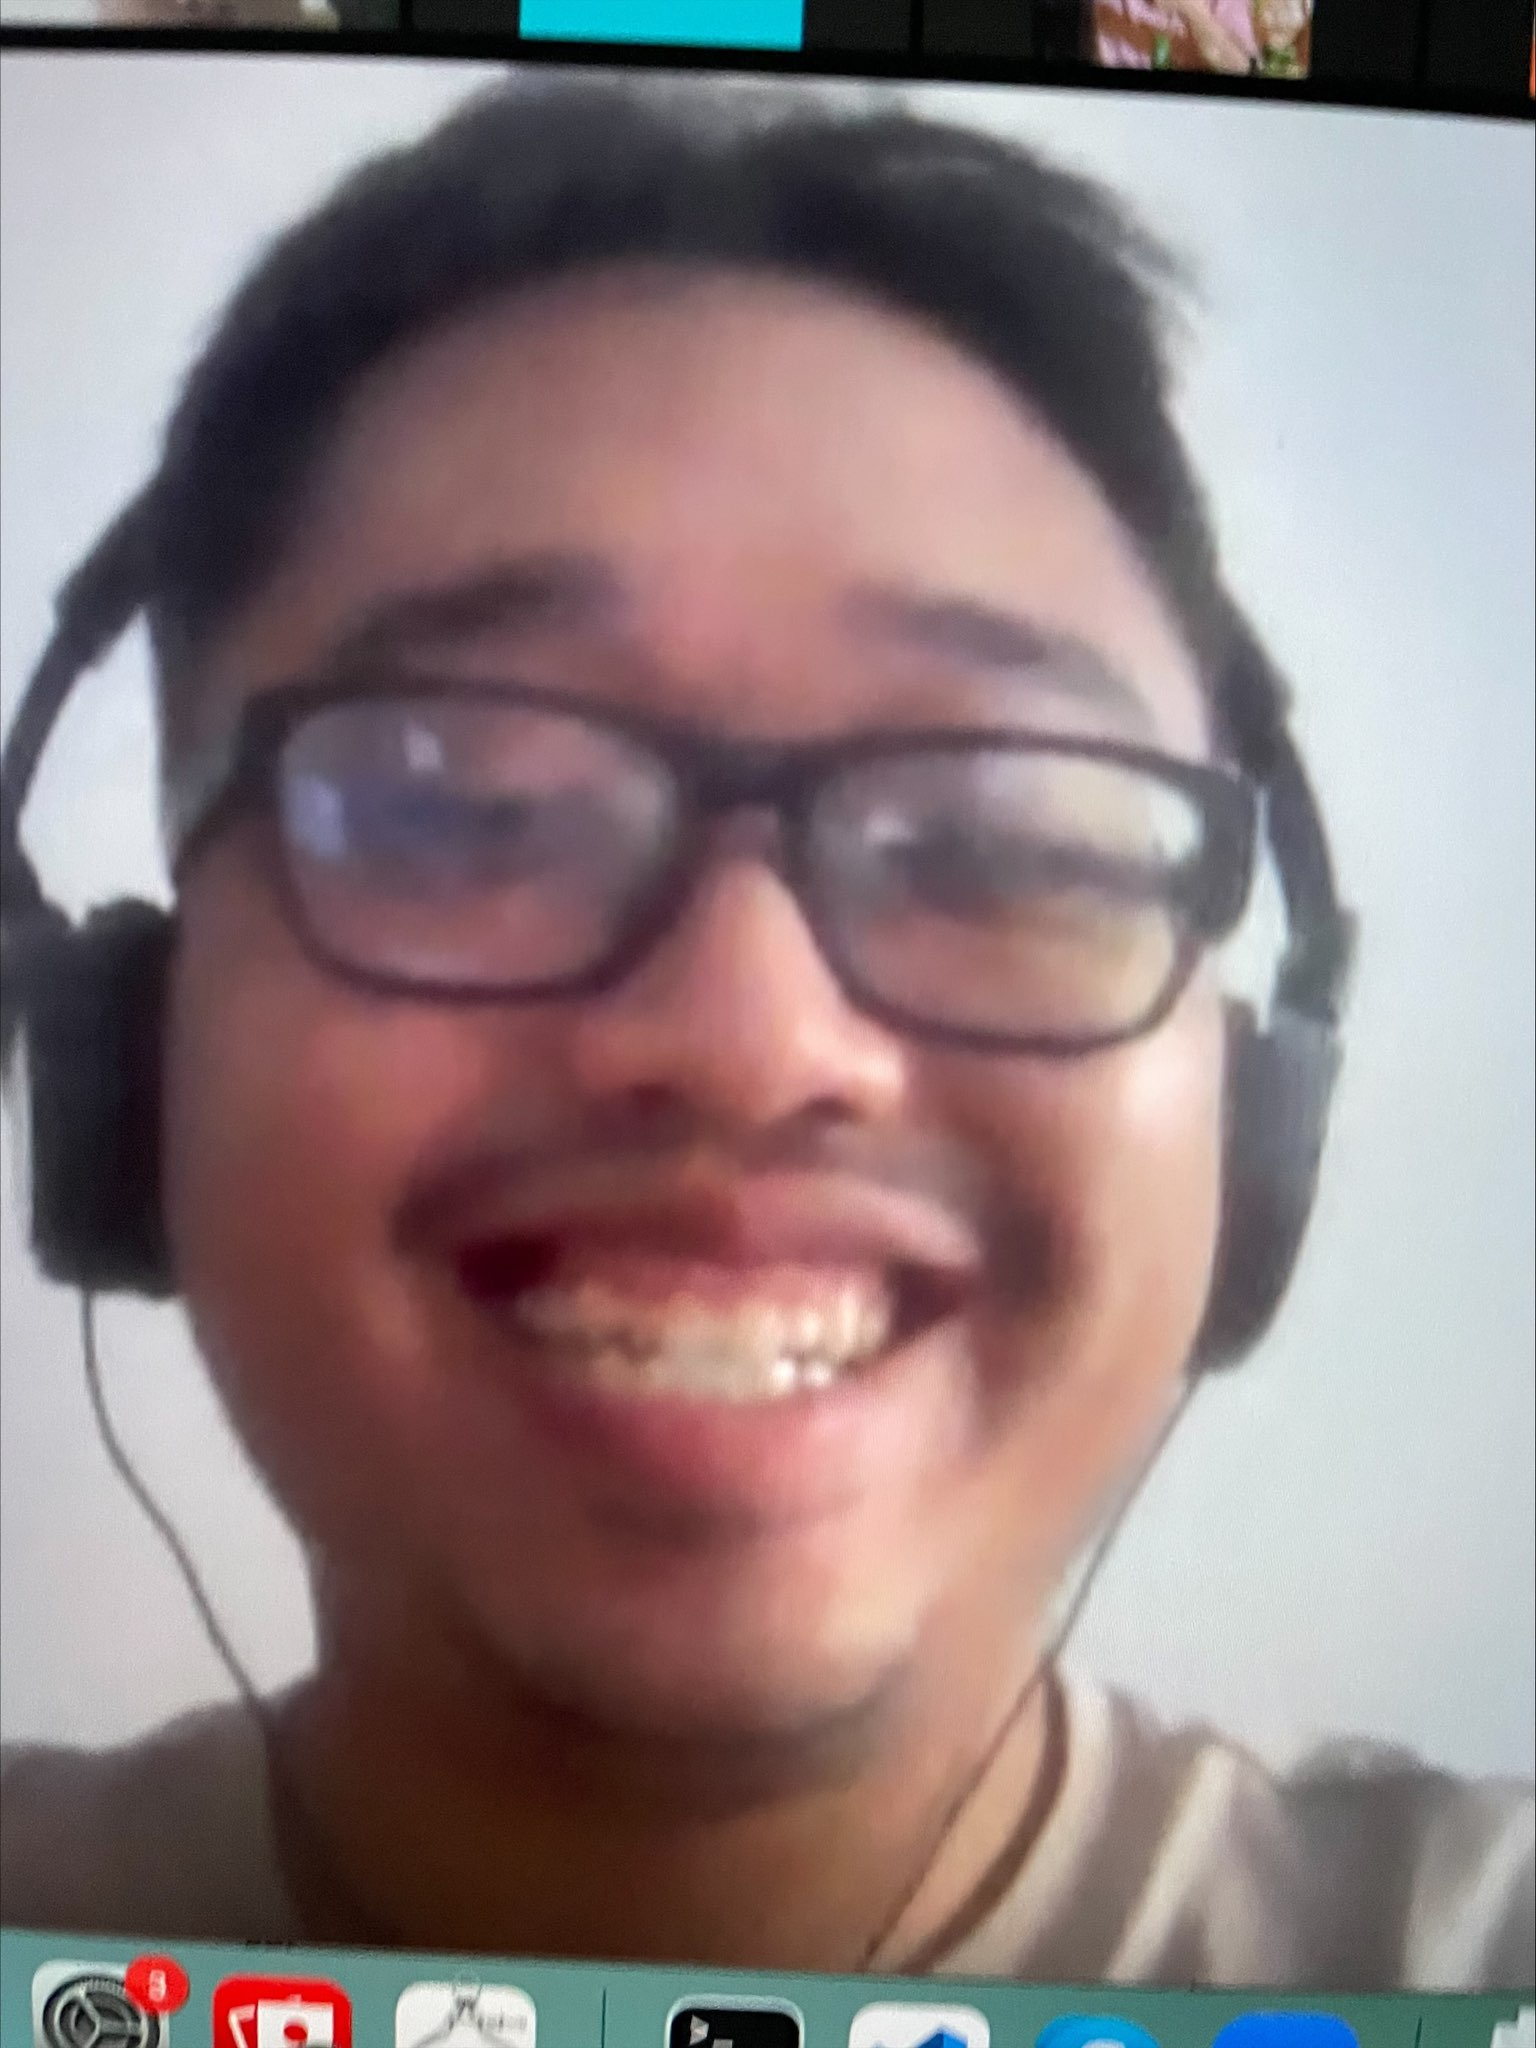
\includegraphics[width=0.5\textwidth]{images/test.jpg}
    \caption{Original RGB photo}
    \label{fig:test}
\end{figure}

As you can see in the figure \ref{fig:test}, the image is RGB originally. After implementation of Kuwahara code with CPU/GPU, the resulting image is an animated picture.

\section*{Implementations}


% code from http://rosettacode.org/wiki/Fibonacci_sequence#Python
\begin{lstlisting}[caption= Sample Python code -- gray scale RGB image 1D and 2D implementations.]

# CPU implementation
def Kuwahara(image, size, v_= None):

    image = image.astype(np.float64)
    output = np.zeros(image.shape)
    mean = np.zeros([4, image.shape[0],image.shape[1]])
    std = mean.copy()

    kernel_template = np.hstack((np.ones((1,int((size-1)/2)+1)),np.zeros((1,int((size-1)/2)))))
    # =====
    # [[1. 1. 1. 0. 0.]]
    pad = np.zeros((1,size))
    # =====
    # [[0. 0. 0. 0. 0.]]
    kernel = np.tile(kernel_template, (int((size-1)/2)+1,1))
    # =====
    # [[1. 1. 1. 0. 0.]
    # [1. 1. 1. 0. 0.]
    # [1. 1. 1. 0. 0.]]
    kernel = np.vstack((kernel, np.tile(pad, (int((size-1)/2),1))))
    # =====
    # [[1. 1. 1. 0. 0.]
    # [1. 1. 1. 0. 0.]
    # [1. 1. 1. 0. 0.]
    # [0. 0. 0. 0. 0.]
    # [0. 0. 0. 0. 0.]]
    # =====
    average = kernel/np.sum(kernel)
    # =====
    # [[0.11111111 0.11111111 0.11111111 0.         0.        ]
    # [0.11111111 0.11111111 0.11111111 0.         0.        ]
    # [0.11111111 0.11111111 0.11111111 0.         0.        ]
    # [0.         0.         0.         0.         0.        ]
    # [0.         0.         0.         0.         0.        ]]
    # ====
    
    kernelstack = np.empty((4,size,size)) 
    kernelstack[0] = average			              # a
    kernelstack[1] = np.fliplr(average)	        # b
    kernelstack[2] = np.flipud(average)	        # c
    kernelstack[3] = np.fliplr(kernelstack[2])	# d
    
    # [ a  a  ab   b  b]
    # [ a  a  ab   b  b]
    # [ac ac abcd bd bd]
    # [ c  c  cd   d  d]
    # [ c  c  cd   d  d]

    for i in range(4):
        mean[i] = conv2d(image, kernelstack[i]) 	                 # mean 
        std[i] = conv2d(image**2, kernelstack[i]) - mean[i]**2 		 # variance         

    if v_ is not None:
      indices = np.argmin(v_,0) 
      for i in range(image.shape[0]):
          for k in range(image.shape[1]):
              output[i,k] = mean[indices[i,k], i,k].astype('uint8')
    else:
      indices = np.argmin(std,0) 

      for i in range(image.shape[0]):
          for k in range(image.shape[1]):
              output[i,k] = mean[indices[i,k], i,k]

    return output, std


  
\end{lstlisting}



\begin{lstlisting}[caption=Averaging Kernel preparation]

    # =====
    # [[0.11111111 0.11111111 0.11111111 0.         0.        ]
    # [0.11111111 0.11111111 0.11111111 0.         0.        ]
    # [0.11111111 0.11111111 0.11111111 0.         0.        ]
    # [0.         0.         0.         0.         0.        ]
    # [0.         0.         0.         0.         0.        ]]
    # ====
    
    kernelstack = np.empty((4,size,size)) 
    kernelstack[0] = average			              # a
    kernelstack[1] = np.fliplr(average)	        # b
    kernelstack[2] = np.flipud(average)	        # c
    kernelstack[3] = np.fliplr(kernelstack[2])	# d
    
    # [ a  a  ab   b  b]
    # [ a  a  ab   b  b]
    # [ac ac abcd bd bd]
    # [ c  c  cd   d  d]
    # [ c  c  cd   d  d]

\end{lstlisting}

\begin{quote}
\textbf{Averaging kernel:\\}
In this method we do not need to run pixel by pixel but rather convolve the image!  \\
In turn, all of the filters (a, b, c, d) will be prepared as above and multiply with the padded images, resulting in std calculation, RGB output.
\end{quote}

To be able to get STD of V in HSV we implement the RGB to HSV conversion code:

\begin{lstlisting}[caption=rgb to hsv]

def rgb_to_hsv(r, g, b):
    r, g, b = r/255.0, g/255.0, b/255.0
    mx = max(r, g, b)
    mn = min(r, g, b)
    df = mx-mn
    # print(mx)
    if mx == mn:
        h = 0.0
    elif mx == r:
        h = 60*((g-b)/df % 6)
    elif mx == g:
        h = 60*((b-r)/df + 2)
    elif mx == b:
        h = 60*((r-g)/df + 4)
    if mx == 0.0:
        s = 0.0
    else:
        s = (df/mx)
    v = mx
    return h, s, v

\end{lstlisting}


\begin{figure}[h]
    \centering
    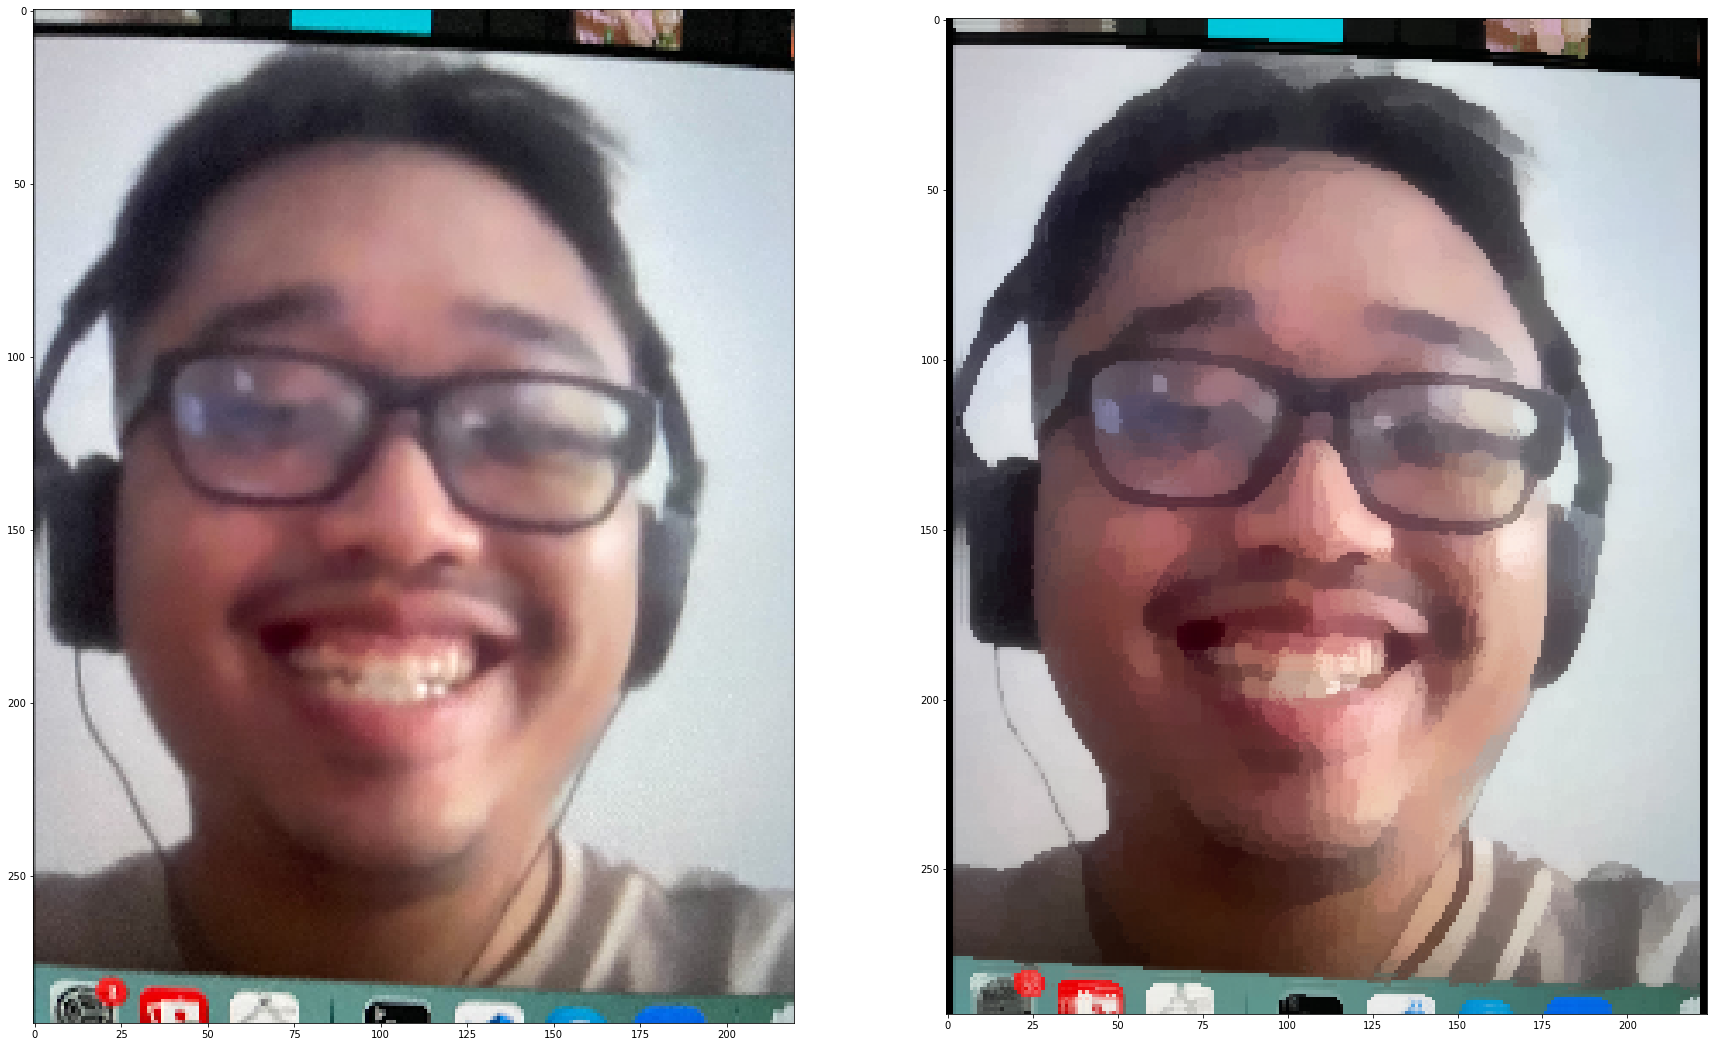
\includegraphics[width=1\textwidth]{images/CPU.png}
    \caption{On the left: Original image, On the right: Filtered image}
    \label{fig:CPU}
\end{figure}

\section*{GPU implementation code}

\begin{lstlisting}[caption=RGB to HSV conversion with GPU]

@cuda.jit
def rgb_to_hsv(in_, out):
    x = cuda.threadIdx.x + cuda.blockIdx.x * cuda.blockDim.x
    y = cuda.threadIdx.y + cuda.blockIdx.y * cuda.blockDim.y
    r, g, b = in_[x, y, 0], in_[x, y, 1], in_[x, y, 2]
    mx = max(r, g, b)
    mn = min(r, g, b)
    df = mx-mn

    if mx == mn:
        h = 0.0
    elif mx == r:
        h = 60*((g-b)/df % 6)
        
    elif mx == g:
        h = 60*((b-r)/df + 2)
        
    elif mx == b:
        h = 60*((r-g)/df + 4)
        
    if mx == 0.0:
        s = 0.0
    else:
        s = (df/mx)
    v = mx

    out[0, x, y] = h 
    out[1, x, y] = s
    out[2, x, y] = v
\end{lstlisting}



\begin{quote}
\textbf{RGB to HSV in GPU\\}
Here we keep the similar code but manage the memory of GPU to run in parallel.
\end{quote}




\begin{lstlisting}[caption=Kuwahara using V value from HSV]

@cuda.jit
def Kuwahara_v(RGB, V_in, KuwaRGB, kernelSize):
    tidx = cuda.threadIdx.x + cuda.blockIdx.x * cuda.blockDim.x
    tidy = cuda.threadIdx.y + cuda.blockIdx.y * cuda.blockDim.y
    # Memory management is the most counter-intuitive part of this project
    kernel_map = (
                ((tidx-kernelSize, tidx+1), (tidy-kernelSize, tidy+1)),
                ((tidx, tidx+kernelSize+1), (tidy-kernelSize, tidy+1)),
                ((tidx-kernelSize, tidx+1), (tidy, tidy+kernelSize+1)),
                ((tidx, tidx+kernelSize+1), (tidy, tidy+kernelSize+1))
                )
    min_std = 99999.0
    min_idx = 0
    for idx in range(4):
    
        # Previously this part was CPU implementation.
        # mean[i] = conv2d(image, kernelstack[i]) 	                 # mean 
        # std[i] = conv2d(image**2, kernelstack[i]) - mean[i]**2     # variance
        # y, x = image.shape
        # y = y - height + 1
        # x = x - height + 1
        # new_image = np.zeros((y ,x))
        # print (new_image.shape)

        # Now convolution and STD calculation will be conducted in parallel as below
        sum = 0.0
        sumSquare = 0.0
        for wi in range(*kernel_map[idx][0]):
          for wj in range(*kernel_map[idx][1]):
                sum += V_in[2,wi, wj]
                sumSquare += V_in[2, wi, wj] **2
        
        mean = sum/(kernelSize+1)**2
        std = math.sqrt(abs(sumSquare /(kernelSize+1)**2 - mean**2))
        if std < min_std:
            min_std = std
            min_idx = idx

    # After STD calculation we can use the V with minimum STD to get the average of RGB value inside of the kernel
    sum_r = 0.0
    sum_g = 0.0
    sum_b = 0.0
    for i in range(*kernel_map[min_idx][0]):
        for j in range(*kernel_map[min_idx][1]):
            sum_r += RGB[i, j, 0]
            sum_g += RGB[i, j, 1]
            sum_b += RGB[i, j, 2]
    
    # Average of RGB with V index and return to output
    KuwaRGB[tidx, tidy, 0] = sum_r / (kernelSize+1)**2
    KuwaRGB[tidx, tidy, 1] = sum_g / (kernelSize+1)**2
    KuwaRGB[tidx, tidy, 2] = sum_b / (kernelSize+1)**2
    
\end{lstlisting}

\begin{quote}
\textbf{Kuwahara in GPU\\}
Here the result ! a little too big kernel size!
Memory management is the most counter-intuitive part of this project, while convolution in GPU is the most mind bending experience!
\end{quote}

\begin{figure}[h]
    \centering
    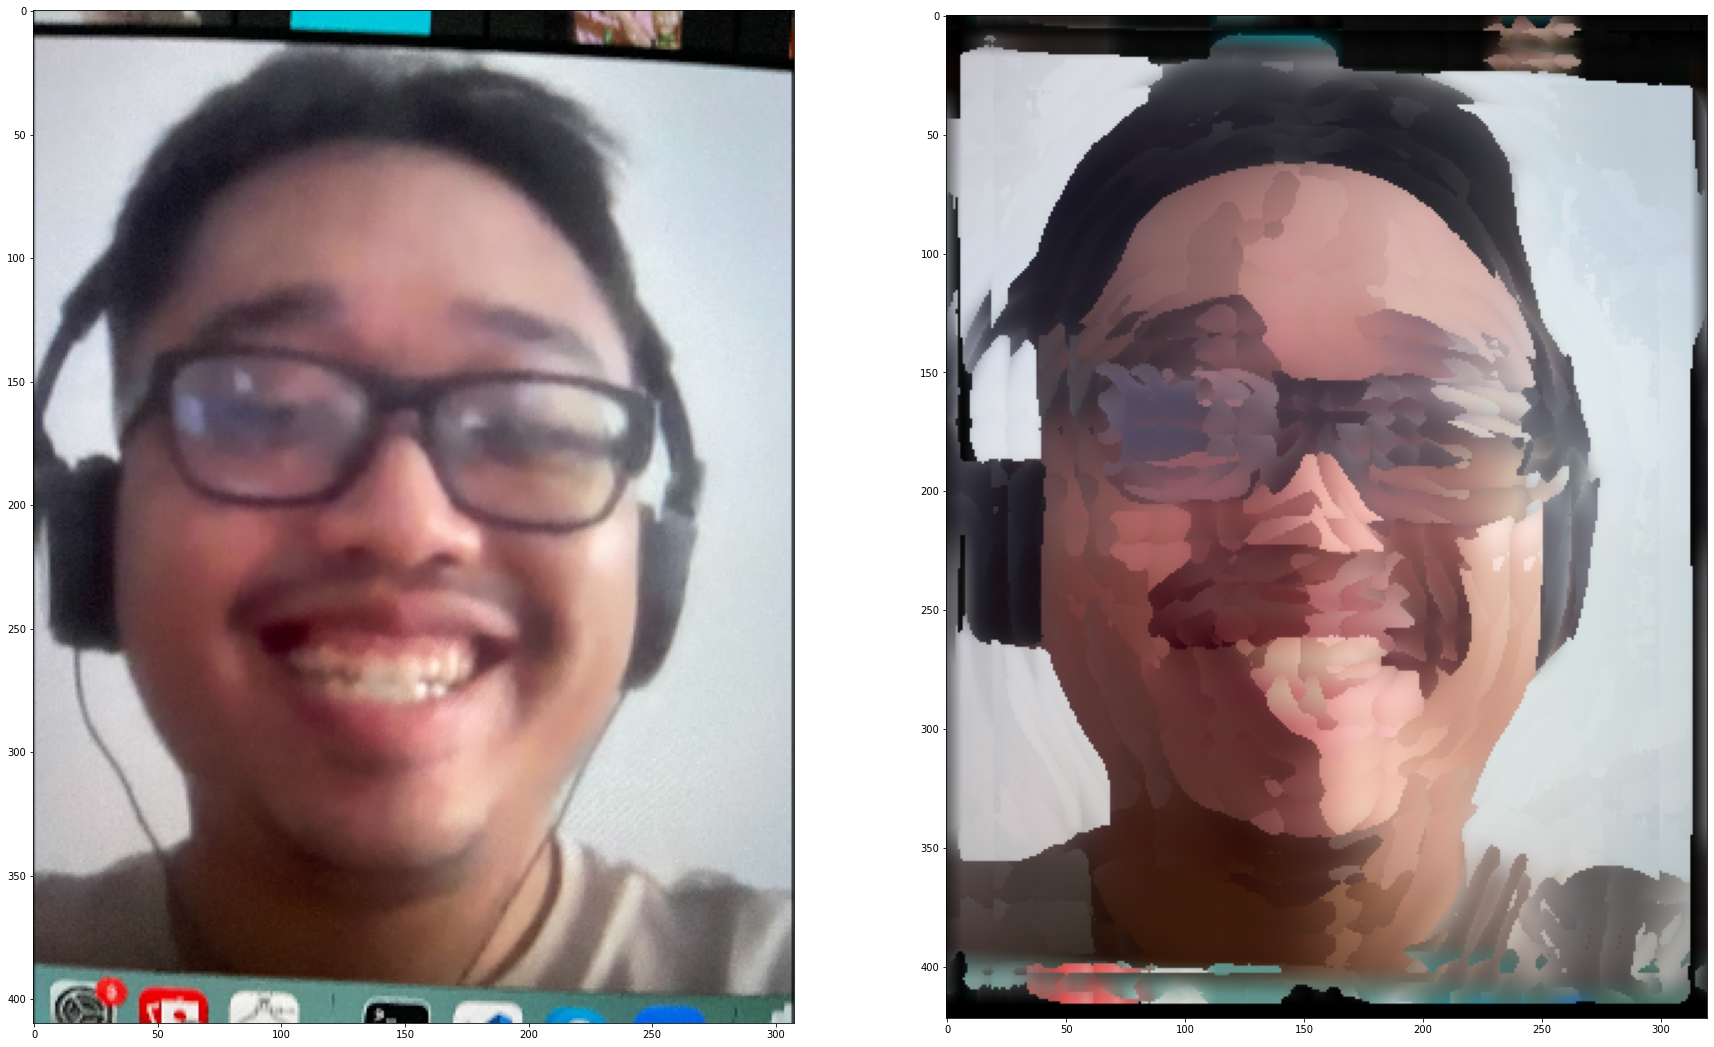
\includegraphics[width=1\textwidth]{images/GPU.png}
    \caption{On the left: Original image, On the right: Filtered image with GPU}
    \label{fig:GPU}
\end{figure}

\end{document}
